\documentclass[conference,10pt,letterpaper]{IEEEtran}
\usepackage[T1]{fontenc}
\usepackage[utf8]{inputenc}
\usepackage{cite}
\usepackage{amsmath,amssymb}
\usepackage{graphicx}
\usepackage{booktabs}
\usepackage{microtype}
\usepackage{url}
\usepackage[hidelinks]{hyperref}
% Generated from pinned per-seed evidence; AUC percent / gain percentage points.
\newcommand{\MinDegradationGain}{5.53}
\newcommand{\MaxDegradationGain}{12.96}
\newcommand{\PositiveDegradationPairs}{30}
\newcommand{\PureMinimum}{49.55}
\newcommand{\PureMaximum}{55.41}
\newcommand{\ResnetCleanStandard}{88.45}
\newcommand{\ResnetCleanRobust}{84.87}
\newcommand{\ResnetCleanGain}{-3.57}
\newcommand{\ResnetDegradedStandard}{66.47}
\newcommand{\ResnetDegradedRobust}{76.90}
\newcommand{\ResnetDegradedGain}{10.42}
\newcommand{\ResnetExternalStandard}{70.00}
\newcommand{\ResnetExternalRobust}{67.98}
\newcommand{\ResnetExternalGain}{-2.02}
\newcommand{\ResnetExternalGainAbs}{2.02}
\newcommand{\ResnetCleanGainAbs}{3.57}
\newcommand{\MobileCleanStandard}{84.70}
\newcommand{\MobileCleanRobust}{83.12}
\newcommand{\MobileCleanGain}{-1.58}
\newcommand{\MobileDegradedStandard}{67.00}
\newcommand{\MobileDegradedRobust}{74.89}
\newcommand{\MobileDegradedGain}{7.89}
\newcommand{\MobileExternalStandard}{69.84}
\newcommand{\MobileExternalRobust}{70.10}
\newcommand{\MobileExternalGain}{0.27}
\newcommand{\MobileExternalGainAbs}{0.27}
\newcommand{\MobileCleanGainAbs}{1.58}
\newcommand{\XceptionCleanStandard}{77.29}
\newcommand{\XceptionCleanRobust}{75.45}
\newcommand{\XceptionCleanGain}{-1.84}
\newcommand{\XceptionDegradedStandard}{62.97}
\newcommand{\XceptionDegradedRobust}{68.50}
\newcommand{\XceptionDegradedGain}{5.53}
\newcommand{\XceptionExternalStandard}{73.94}
\newcommand{\XceptionExternalRobust}{67.18}
\newcommand{\XceptionExternalGain}{-6.77}
\newcommand{\XceptionExternalGainAbs}{6.77}
\newcommand{\XceptionCleanGainAbs}{1.84}
\newcommand{\VitCleanStandard}{81.43}
\newcommand{\VitCleanRobust}{82.27}
\newcommand{\VitCleanGain}{0.84}
\newcommand{\VitDegradedStandard}{69.25}
\newcommand{\VitDegradedRobust}{76.39}
\newcommand{\VitDegradedGain}{7.14}
\newcommand{\VitExternalStandard}{69.93}
\newcommand{\VitExternalRobust}{72.29}
\newcommand{\VitExternalGain}{2.36}
\newcommand{\VitExternalGainAbs}{2.36}
\newcommand{\VitCleanGainAbs}{0.84}
\newcommand{\ClipCleanStandard}{91.95}
\newcommand{\ClipCleanRobust}{90.75}
\newcommand{\ClipCleanGain}{-1.20}
\newcommand{\ClipDegradedStandard}{74.89}
\newcommand{\ClipDegradedRobust}{84.53}
\newcommand{\ClipDegradedGain}{9.65}
\newcommand{\ClipExternalStandard}{75.15}
\newcommand{\ClipExternalRobust}{81.19}
\newcommand{\ClipExternalGain}{6.04}
\newcommand{\ClipExternalGainAbs}{6.04}
\newcommand{\ClipCleanGainAbs}{1.20}
\newcommand{\DinoCleanStandard}{93.58}
\newcommand{\DinoCleanRobust}{92.69}
\newcommand{\DinoCleanGain}{-0.89}
\newcommand{\DinoDegradedStandard}{71.47}
\newcommand{\DinoDegradedRobust}{84.44}
\newcommand{\DinoDegradedGain}{12.96}
\newcommand{\DinoExternalStandard}{71.46}
\newcommand{\DinoExternalRobust}{77.92}
\newcommand{\DinoExternalGain}{6.46}
\newcommand{\DinoExternalGainAbs}{6.46}
\newcommand{\DinoCleanGainAbs}{0.89}

\graphicspath{{generated/}}
\newcommand{\testd}{Test-D}
\newcommand{\auc}{\operatorname{AUC}}
\newcommand{\std}{\mathrm{std}}
\newcommand{\rob}{\mathrm{rob}}
\title{When Robustness Does Not Transfer:\\Spatial and Spectral Cues for Face Forgery Detection}
\author{\IEEEauthorblockN{Lucas Cunha, Lucas Sotomaior, Lucas Gasperin, Beatriz Caldas, Eduardo Pianovski, Rayson Laroca}
\IEEEauthorblockA{Pontifical Catholic University of Paran\'a, Curitiba, Brazil\\
\{c.oliveira25,lucas.sotomaior,lucas.gasperin,beatriz.caldas,eduardo.pianovski\}@pucpr.edu.br\\
rayson@ppgia.pucpr.br}}
\begin{document}
\maketitle

\begin{abstract}
Face forgery detectors can improve on degraded images without becoming more transferable to another dataset. We investigate this distinction through a reproducible reanalysis of released experiments on the Multi-Dimensional Face Forgery Image (MFFI) benchmark. The primary evidence comprises 210 fine-tuned configurations spanning six model families, seven spatial or spectral representations, and five seeds, together with 30 robustly trained RGB runs on the same seed set. We recompute clean-test and degraded-test summaries and pair the RGB runs with their reported evaluations on a DF40-derived local subset. Robust training improves MFFI Test-D AUC in all \PositiveDegradationPairs{} architecture--seed pairs, with architecture-level gains of \MinDegradationGain{}--\MaxDegradationGain{} percentage points. Transfer behaves differently: CLIP and DINOv3 improve by \ClipExternalGain{} and \DinoExternalGain{} points, whereas Xception declines by \XceptionExternalGainAbs{} points despite improving on Test-D. Pure-frequency representations achieve only \PureMinimum{}--\PureMaximum{}\% mean Test-D AUC under the evaluated pipeline; selected hybrid inputs provide smaller, architecture-dependent gains. Separate ensemble summaries favor a CLIP--DINOv3 pair over indiscriminate six-model fusion, but are not pooled with the primary seed cohort. These findings support evaluating degradation tolerance, representation choice, and dataset transfer as distinct properties. We release the seed-level reconciliation, generated tables, and explicit provenance limits rather than interpreting a single robustness score as general forensic reliability.
\end{abstract}
\begin{IEEEkeywords}
Face forgery detection, deepfake detection, robustness, distribution shift, frequency representations, reproducible evaluation.
\end{IEEEkeywords}

\section{Introduction}
A face forgery detector is useful only if its decisions survive the conditions under which an image is encountered. A classifier may distinguish the training collection accurately and still rely on cues that change after processing or disappear in another collection. Frequency statistics, pretrained visual representations, and augmentation offer different ways to address this problem~\cite{frank2020,wang2020,ojha2023}. Their benefits, however, need not appear under the same evaluation shift. Better discrimination on a degraded test set is not, by itself, evidence of better transfer to different sources or forgery methods.

This distinction matters when interpreting modern benchmarks. MFFI varies authentic-image sources, forgery types, and test-time degradation~\cite{miao2025}. DF40 expands the range of forgery techniques and evaluation protocols~\cite{yan2024df40}. Both are more informative than a clean-set score alone, but neither makes ``generalization'' a single measurable quantity. Source composition, degradation, input representation, and training policy can all change at once. Following the broader motivation of distribution-shift benchmarks~\cite{koh2021}, we ask a narrower question: \emph{when a training regime improves degraded-image discrimination, which of those improvements persist under dataset transfer?}

We examine this question using the latest released experiments of our spatial--spectral face-forgery benchmark, extending the scope of the preceding study~\cite{cunha2026}. The analysis covers ResNet-18, MobileNetV3-Large, Xception, ViT-B/16, CLIP ViT-B/16, and DINOv3 ConvNeXt-Base. Seven input representations distinguish RGB, four pure-frequency encodings, and two spatial--spectral concatenations. A second collection applies stronger augmentation to RGB training. Instead of comparing inconsistent summary rows, we align the primary experiments on the same five seeds and recompute their means, dispersion, and paired differences from the released records.

The main result is a separation between two outcomes often described by the same word. Robust RGB training improves \testd{} AUC for every architecture and every included seed. Yet the corresponding DF40-subset comparison is not uniformly positive: ResNet and Xception lose mean transfer AUC, MobileNet changes little, and the pretrained CLIP and DINOv3 models gain. Within the standard training matrix, replacing RGB with a pure-frequency input also fails to provide a generally stronger degraded-image detector. Hybrid inputs produce exceptions, not a universal ordering.

Our contribution is an empirical characterization of these distinctions, not a new detection architecture. First, we provide a complete, seed-matched comparison of clean performance, degradation tolerance, and recorded dataset transfer. Second, we contextualize that comparison within the full representation matrix, retaining negative results and separating weak initial discrimination from robustness. Third, we reconcile the scope of the primary results with the separate ensemble and explanation artifacts, so that cohort differences and illustrative evidence do not become unsupported headline claims. The accompanying analysis regenerates the numerical tables and claim values from a pinned release~\cite{release2026}.

The resulting conclusion is deliberately specific. For the evaluated pipelines, a stronger augmented RGB model is a more useful baseline than the assumption that spectral inputs are inherently robust. Even that stronger baseline requires a separate transfer evaluation. The experiments do not establish robustness to all manipulations, causal explanations of the learned features, or state-of-the-art performance under unmatched published protocols.

\section{Related Work}
\subsection{Benchmark design and the meaning of transfer}
DeepfakeBench identifies inconsistent preprocessing, experimental settings, and evaluation as obstacles to meaningful detector comparison~\cite{yan2023bench}. DF40 further shows why a detector ranked highly under a restricted train--test protocol may not address a broader forgery space~\cite{yan2024df40}. MFFI combines multiple forgery categories with heterogeneous authentic sources and a degraded test partition~\cite{miao2025}. We use these works to distinguish an evaluation condition from a claim of universal generalization. In particular, our local DF40 export is not equated with every official DF40 protocol, and clean MFFI testing is not assumed to be identically distributed with training.

This framing is consistent with WILDS, which treats domain definition and evaluation design as part of the benchmark rather than incidental implementation details~\cite{koh2021}. Our study is smaller in scope: it analyzes one released face-forgery experiment collection and its external evaluation records. It does not estimate performance over a population of all possible datasets.

\subsection{Spatial, spectral, and pretrained representations}
Frequency analysis can expose regularities of image generation that are less apparent in the spatial image~\cite{frank2020}. Such usefulness is conditional on the representation and training setting. FreqDebias, for example, addresses spectral bias with frequency-aware augmentation and consistency objectives~\cite{kashiani2025}; it is not simply a classifier trained on an FFT magnitude image. Consequently, a negative result for our magnitude, phase, or complex-input baselines cannot refute frequency-aware detection as a whole.

Wang et al. show the importance of training choices, including processing-based augmentation, when testing generated-image detection beyond a training generator~\cite{wang2020}. Ojha et al. demonstrate a different route through pretrained features and simple classifiers~\cite{ojha2023}. CLIP learns transferable visual representations using language supervision~\cite{radford2021}, while DINOv3 provides self-supervised visual models~\cite{simeoni2025}. We evaluate fine-tuned classifiers built on these families, not a reproduction of CLIP zero-shot detection or a frozen-feature universal-detector protocol. Nor is architecture isolated from pretraining data, model size, or fine-tuning policy. Our comparisons concern the implemented systems.

\subsection{Explanations require a separate evaluation}
A plausible saliency map does not establish why one model transfers better. Integrated Gradients (IG) and Grad-CAM answer different attribution questions~\cite{sundararajan2017,selvaraju2017}, and the appearance of a map alone is insufficient to assess dependence on learned parameters~\cite{adebayo2018}. The distinction between explanatory appearance and an evaluated explanation is central to rigorous interpretability research~\cite{doshi2017}. We therefore separate the existing qualitative gallery from the quantitative detection results and describe the controls needed for a stronger mechanism-oriented analysis.

\section{Experimental Scope and Evidence}
\subsection{Data and evaluation conditions}
\label{sec:data}
We study binary image classification with $y=0$ for real images and $y=1$ for forgeries. MFFI is the source benchmark. Table~\ref{tab:population} gives the exact counts in the released CSV manifests, rather than rounding them to the dataset paper's nominal totals. The three manifests contain no duplicate image filenames within a split and no exact filename overlap across splits. This is a filename-level check, not evidence of disjoint identities, independent video frames, or absence of near-duplicate content.

\begin{table}[t]
\caption{Exact MFFI manifest counts in the pinned release. Counts describe the manifests, not independently verified image-level coverage for every historical run.}
\label{tab:population}
\centering
\small
\begin{tabular}{lrrr}
\toprule
Partition & Real & Fake & Total \\
\midrule
Train & 99,386 & 425,043 & 524,429 \\
Validation & 59,082 & 88,281 & 147,363 \\
Clean test & 77,602 & 104,345 & 181,947 \\
\bottomrule
\end{tabular}

\end{table}

We distinguish three conditions. \emph{Clean test} denotes the provided MFFI test partition without the additional Test-D processing. It is not an i.i.d. claim: the original dataset deliberately varies authentic sources across its partitions~\cite{miao2025}. \emph{Test-D} is MFFI's degraded test condition. The dataset design includes conventional processing disturbances and patch-based adversarial perturbations; the released per-run AUC records do not identify each image's realized operation or severity. We therefore analyze the reported aggregate condition, not a corruption-specific response curve or robustness against a newly optimized adaptive attack. \emph{Dataset transfer} denotes evaluation of the MFFI-trained systems on the project's DF40-derived local subset.

The external subset requires a qualification. The accompanying preparation code samples selected available folders, pools chosen authentic sources, and skips missing folders. Its manifest and per-image membership are not included with the aggregate records analyzed here. We accordingly use ``DF40 subset'' throughout, do not assert complete official coverage, and do not attribute a transfer difference solely to unseen generators. Source-image composition, extraction, and preprocessing may also contribute. This limitation does not erase the recorded contrast between Test-D gains and transfer losses, but it bounds that contrast to the released local evaluation.

\subsection{A fixed primary seed population}
\label{sec:population}
The primary seed set is
\begin{equation}
\mathcal{S}=\{7,42,123,2024,2025\}.
\end{equation}
The standard fine-tuning table contains exactly one row for every combination of six families, seven representations, and these five seeds: 210 configurations in total. The robust-training exports contain 30 RGB rows, one for every family--seed pair. We join the two collections by family and seed and separately join the RGB standard runs to the seed-level DF40 evaluation table. No seed is imputed, duplicated, or replaced after examining its score.

Seed 987 is not part of this primary comparison. Earlier robust-training code constructs an unsuffixed fine-tuning run and can store its output under that regime's path. Combining such records with nominal standard runs would make a directory label insufficient to identify the training treatment. The chosen primary cohort instead follows the complete standard matrix and its matching robust exports. This is a retrospective inclusion rule based on record structure, not a claim of preregistration.

The ensemble collection is secondary evidence. It reports five-seed summaries, but does not supply the constituent rows needed to reconcile every aggregate to $\mathcal{S}$; the same collection includes self-ensemble member lists containing seed 987. We therefore preserve its reported means and dispersion in a separate table rather than pool them with the recomputed primary results. A five-member self-ensemble is one combined predictor, not five independent evaluations of that predictor.

\subsection{Provenance and reproducibility boundary}
All evidence is frozen at source revision \texttt{d156d7789728}~\cite{release2026}. The analysis verifies source-file Git identities, checks the complete experimental grid, and generates its tables, figure, and numerical text values directly from the selected records. Robust per-seed metrics were exported to four decimal places, so recomputation does not recover additional measurement precision.

The present work adds analysis, not new detector training. The available evidence supports reproducing the numerical aggregation, but does not independently reproduce each historical model prediction. Complete checkpoint hashes, resolved run configurations, external manifests, and per-example outputs are not available for all included runs. We use the released implementation to describe the intended pipeline and explicitly distinguish those settings from an independently verified training history. The original result files remain unchanged; the accompanying reconciliation documents exclusions rather than silently repairing incompatible summaries.

\section{Models, Representations, and Analysis}
\subsection{Detector families and input construction}
The evaluated families are ResNet-18~\cite{he2016}, MobileNetV3-Large~\cite{howard2019}, Xception~\cite{chollet2017}, ViT-B/16~\cite{dosovitskiy2021}, CLIP ViT-B/16~\cite{radford2021}, and DINOv3 ConvNeXt-Base~\cite{simeoni2025}. The DINOv3 configuration uses a ConvNeXt backbone; its results must not be interpreted as a comparison of two vision-transformer architectures against convolutional networks. Each family is adapted for two-class prediction, and the input projection is adapted to the selected number of channels.

The standard matrix contains seven named representations. RGB retains the three spatial channels. Magnitude, phase, complex, and high-pass modes provide only frequency-domain inputs. RGB+M concatenates RGB with spectral magnitude. The hybrid mode concatenates RGB with several spectral maps. In the released encoder, the image is resized to the configured spatial resolution, converted to luminance, and transformed by a centered two-dimensional FFT,
\begin{equation}
F=\operatorname{fftshift}\bigl(\operatorname{FFT2}(0.299R+0.587G+0.114B)\bigr).
\end{equation}
Magnitude uses log compression and per-image range normalization; phase is scaled by its angular range. The complex representation retains real and imaginary components with a shared magnitude scale. The high-pass representation suppresses the central frequency disk before magnitude compression. RGB uses ImageNet channel normalization.

The current hybrid encoder outputs RGB, magnitude, phase, high-pass, and low-pass channels; compatibility code also supports earlier channel layouts. Since historical summary rows do not resolve every layout version, we report the released mode identifiers rather than claim that all historical hybrids have an independently verified channel contract. These are global frequency-coordinate inputs, not spatial maps of where a face was manipulated. Concatenating spectral bins with RGB pixels likewise does not make their coordinates physically equivalent.

\subsection{Standard and robust training regimes}
The standard RGB transform uses random resized cropping, horizontal flipping, and modest color jitter. In the released standard entry point, non-RGB modes instead follow a resize-based path without the same random augmentation. Thus the seven-mode experiment compares the released pipelines; it is not a fully factorial test isolating input representation from augmentation. This distinction is essential when interpreting weak spectral results.

The robust RGB path uses stronger, stochastic image-space processing. Random resized cropping uses a scale range of $[0.8,1.0]$, followed by horizontal flipping. Rotation, contrast, brightness, JPEG compression, and Gaussian noise are each enabled with probability $0.5$; sharpness and Gaussian blur use probability $0.3$. Rotation spans $[-30^\circ,30^\circ]$; contrast and brightness factors span $[0.4,1.8]$ and $[0.5,1.8]$. Sharpness spans $[0.2,2.0]$, blur radius $[0.5,2.0]$, JPEG quality $[25,90]$, and additive-noise standard deviation $[0.01,0.08]$ on the unit-scaled tensor. Noise is clipped to the valid input range before normalization. The implementation does not contain the H.264 or motion-blur operations sometimes associated with generic descriptions of robust preprocessing.

The released configuration defaults use $224\times224$ inputs, including Xception, and a two-class cross-entropy objective. The trainer uses AdamW, validation-AUC checkpoint selection, and a validation-driven learning-rate scheduler. Family-specific settings differ: the base configuration allows 50 epochs, whereas CLIP and Xception specify 20; CLIP specifies batch size 16 rather than the base 32. DINOv3 also overrides learning rates and enables mixup. The robust launcher accepts additional command-line overrides and explicitly builds a fine-tuning model before training. We therefore refer to a \emph{seed-matched regime comparison}, not an exactly compute-matched or augmentation-only causal intervention. Resolved per-run configurations would be needed to establish the latter.

\subsection{Metrics, paired differences, and uncertainty}
For a system with fake-class score $p(x)$, ROC AUC measures the probability that a randomly selected fake receives a higher score than a randomly selected real, with half credit for ties. We denote the recorded AUC by $A_{m,r,s}^{q}$, for model family $m$, regime $r$, seed $s$, and evaluation condition $q$. The regime difference is computed \emph{within seed}:
\begin{equation}
\delta_{m,s}^{q}=A_{m,\rob,s}^{q}-A_{m,\std,s}^{q},\qquad
\bar\delta_m^{q}=\frac{1}{5}\sum_{s\in\mathcal S}\delta_{m,s}^{q}.
\label{eq:paired}
\end{equation}
We report arithmetic means and sample standard deviations across the five seeds, using denominator $5-1$. Tables express AUC in percent and differences in percentage points (pp). Dispersion of the paired difference is calculated from the five differences, not by combining two marginal standard deviations as if the runs were unpaired.

These standard deviations describe variation across the available runs. They are not confidence intervals over images, identities, or future datasets. The aggregate exports do not support an image- or video-cluster bootstrap for the full primary matrix. We therefore report the direction of each paired change without converting the 30 pairs into independent replications of a population-level hypothesis test. AUC also does not establish calibration, precision at operational prevalence, or an acceptable false-positive rate at a particular decision threshold.

\subsection{Secondary fusion and qualitative evidence}
The ensemble records compare arithmetic score averaging, geometric fusion, and a validation-fitted stacking model. We retain the CLIP--DINOv3 pair and the all-six-family ensemble under all three reported strategies, rather than quote only the maximum external score. Stacking's validation value is a fitting-set statistic unless an independent meta-validation split is available; it should not be treated as an unbiased estimate for selecting among fusion strategies. Exact score definitions and cohort provenance remain part of the release, and the primary conclusions do not depend on an ensemble gain over $\mathcal S$.

The release also contains a two-image Celeb-DF gallery, using a real example and a forged example with selected ResNet, CLIP, and DINO models. Its scripts apply Grad-CAM and/or IG but do not preserve the full raw attribution arrays, numerical residuals, and resolved checkpoint identities needed for a quantitative explanation study. We use the gallery only to motivate the controlled analysis discussed in Section~\ref{sec:explanations}; it does not supply evidence for the main detection claims.

\section{Results}
\subsection{Robust training consistently improves the degraded condition}
\label{sec:robustresults}
Table~\ref{tab:primary} shows the primary RGB comparison. All \PositiveDegradationPairs{} paired Test-D changes are positive. Architecture-level gains range from \MinDegradationGain{} pp for Xception to \MaxDegradationGain{} pp for DINOv3. CLIP increases from \ClipDegradedStandard{}\% to \ClipDegradedRobust{}\% AUC, and DINOv3 from \DinoDegradedStandard{}\% to \DinoDegradedRobust{}\%. The conventional convolutional and ViT baselines also improve; the effect is not confined to the two large-pretraining families.

\begin{table*}[t]
\caption{Primary seed-matched RGB comparison on MFFI. Each AUC cell is mean $\pm$ sample SD over $\mathcal S=\{7,42,123,2024,2025\}$. The last column summarizes the five within-seed robust-minus-standard differences. Values are recomputed from released per-seed records; SD is not a population confidence interval.}
\label{tab:primary}
\centering
\small
\setlength{\tabcolsep}{7pt}
\begin{tabular}{lccccc}
\toprule
Model & \multicolumn{2}{c}{Clean test AUC (\%)} & \multicolumn{2}{c}{Test-D AUC (\%)} & Test-D gain (pp) \\
\cmidrule(lr){2-3}\cmidrule(lr){4-5}
 & Standard & Robust & Standard & Robust & Paired difference \\
\midrule
ResNet-18 & $88.45 \pm 1.13$ & $84.87 \pm 0.84$ & $66.47 \pm 0.87$ & $76.90 \pm 0.73$ & $+10.42 \pm 1.07$ \\
MobileNetV3-L & $84.70 \pm 0.24$ & $83.12 \pm 0.65$ & $67.00 \pm 0.52$ & $74.89 \pm 0.64$ & $+7.89 \pm 0.78$ \\
Xception & $77.29 \pm 0.42$ & $75.45 \pm 0.14$ & $62.97 \pm 0.13$ & $68.50 \pm 0.41$ & $+5.53 \pm 0.36$ \\
ViT-B/16 & $81.43 \pm 0.94$ & $82.27 \pm 0.54$ & $69.25 \pm 0.84$ & $76.39 \pm 0.51$ & $+7.14 \pm 1.06$ \\
CLIP ViT-B/16 & $91.95 \pm 0.41$ & $90.75 \pm 0.15$ & $74.89 \pm 1.03$ & $84.53 \pm 0.24$ & $+9.65 \pm 1.15$ \\
DINOv3 ConvNeXt-B & $93.58 \pm 0.62$ & $92.69 \pm 1.02$ & $71.47 \pm 1.15$ & $84.44 \pm 1.95$ & $+12.96 \pm 1.69$ \\
\bottomrule
\end{tabular}

\end{table*}

The improvement is not free of clean-performance trade-offs. Mean clean AUC decreases for five of the six families. ResNet falls by \ResnetCleanGainAbs{} pp, whereas ViT increases by \VitCleanGain{} pp. DINOv3 retains the highest recorded mean clean AUC among the robust RGB systems, but CLIP and DINOv3 have very similar mean Test-D AUC. Their Test-D run dispersion differs: the corresponding SDs round to $0.24$ and $1.95$ pp. Five seeds do not justify declaring a reliable winner from the small difference between those means.

A narrower clean-to-degraded gap should not be read in isolation. Such a gap can shrink because degraded discrimination improves, because clean discrimination worsens, or both. The side-by-side absolute scores in Table~\ref{tab:primary} expose that distinction. Here, the Test-D improvement is visible directly, while the clean cost remains architecture dependent.

\subsection{The Test-D improvement does not transfer uniformly}
\label{sec:transferresults}
The external comparison changes the interpretation of the robust-training gains. Table~\ref{tab:transfer} reports the same family--seed pairs on the DF40 subset. CLIP improves by \ClipExternalGain{} pp and DINOv3 by \DinoExternalGain{} pp. ViT gains \VitExternalGain{} pp. MobileNet's mean increase is only \MobileExternalGain{} pp, while ResNet and Xception decrease by \ResnetExternalGainAbs{} and \XceptionExternalGainAbs{} pp, respectively.

\begin{table}[t]
\caption{Recorded transfer to the DF40-derived local subset, using the same primary seeds as Table~\ref{tab:primary}. ``Positive pairs'' counts seeds with positive robust-minus-standard AUC. The subset is not asserted to reproduce the complete official DF40 protocol.}
\label{tab:transfer}
\centering
\footnotesize
\setlength{\tabcolsep}{3.5pt}
\begin{tabular}{lcccc}
\toprule
Model & Standard & Robust & Gain & Positive \\
 & \multicolumn{2}{c}{AUC (\%), mean $\pm$ SD} & (pp) & pairs \\
\midrule
ResNet & $70.00 \pm 2.53$ & $67.98 \pm 2.50$ & $-2.02$ & 1/5 \\
MobileNet & $69.84 \pm 0.56$ & $70.10 \pm 1.69$ & $+0.27$ & 4/5 \\
Xception & $73.94 \pm 0.66$ & $67.18 \pm 0.99$ & $-6.77$ & 0/5 \\
ViT & $69.93 \pm 1.20$ & $72.29 \pm 1.99$ & $+2.36$ & 4/5 \\
CLIP & $75.15 \pm 3.85$ & $81.19 \pm 1.32$ & $+6.04$ & 5/5 \\
DINOv3 & $71.46 \pm 2.75$ & $77.92 \pm 3.53$ & $+6.46$ & 4/5 \\
\bottomrule
\end{tabular}

\end{table}

\begin{figure}[t]
\centering
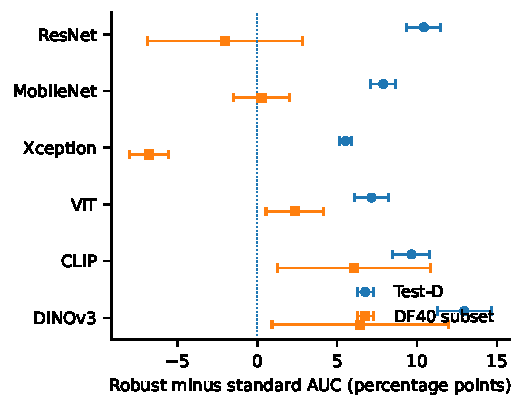
\includegraphics[width=\columnwidth]{augmentation_gains.pdf}
\caption{The two evaluations respond differently to the training regime. Points show mean paired changes; whiskers show sample SD of those changes across five seeds, not confidence intervals. Test-D gains are positive for every family, whereas the DF40-subset change is negative for ResNet and Xception.}
\label{fig:gains}
\end{figure}

Xception is the clearest counterexample to equating the two properties: its Test-D AUC improves in all five seeds while its external AUC declines in all five. ResNet improves on Test-D in all five seeds but on the external subset in only one. CLIP improves in both conditions for every included seed. DINOv3 improves externally in four of five seeds, despite having the largest mean Test-D gain. Figure~\ref{fig:gains} places these differences on the same scale without averaging them into a single robustness index.

These observations do not identify the causal source of a transfer loss. An augmentation may suppress a useful source-specific cue, change optimization, or interact with pretraining and classifier adaptation; the local external pipeline may add another shift. The released records cannot separate those explanations. They do support the operationally relevant statement that the observed Test-D gain is insufficient to predict the sign of the external gain for every detector family.

\subsection{Pure-frequency inputs are weak under the evaluated pipeline}
Table~\ref{tab:representations} places the RGB findings in the full standard fine-tuning matrix. Across the four pure-frequency encodings and six families, mean Test-D AUC ranges from \PureMinimum{}\% to \PureMaximum{}\%. The RGB baselines discriminate more strongly in that condition. Some frequency models are already weak on the clean test, particularly the complex-input CLIP and DINOv3 configurations. A small degradation gap for an almost chance-level detector is not evidence of a useful invariant representation.

\begin{table*}[t]
\caption{The complete standard representation matrix: clean-test / Test-D mean AUC (\%) over the primary five seeds. RGB+M concatenates RGB and FFT magnitude; Hybrid is the release's multi-map spatial--spectral mode. This is a comparison of released pipelines, not an augmentation-matched factorial ablation. Per-seed values and SDs remain available in the analysis export.}
\label{tab:representations}
\centering
\footnotesize
\setlength{\tabcolsep}{5pt}
\begin{tabular}{lccccccc}
\toprule
Model & RGB & Magnitude & Phase & Complex & High-pass & RGB+M & Hybrid \\
\midrule
ResNet & 88.45 / 66.47 & 75.03 / 54.09 & 64.67 / 52.11 & 69.92 / 54.36 & 75.00 / 53.65 & 87.17 / 66.62 & 83.37 / 68.66 \\
MobileNet & 84.70 / 67.00 & 71.77 / 54.20 & 62.87 / 52.34 & 68.72 / 53.37 & 71.27 / 54.52 & 80.49 / 62.96 & 70.84 / 60.32 \\
Xception & 77.29 / 62.97 & 70.35 / 53.28 & 58.89 / 51.11 & 56.22 / 51.74 & 69.94 / 53.30 & 73.29 / 61.19 & 65.92 / 57.46 \\
ViT & 81.43 / 69.25 & 72.40 / 53.47 & 60.20 / 49.55 & 57.01 / 55.41 & 72.40 / 52.81 & 82.65 / 71.23 & 79.15 / 67.56 \\
CLIP & 91.95 / 74.89 & 73.36 / 53.00 & 62.65 / 49.94 & 52.71 / 51.97 & 73.16 / 53.28 & 89.41 / 72.60 & 77.89 / 65.05 \\
DINOv3 & 93.58 / 71.47 & 76.14 / 53.65 & 71.28 / 53.32 & 49.95 / 49.77 & 76.31 / 53.71 & 91.66 / 68.34 & 86.03 / 68.20 \\
\bottomrule
\end{tabular}

\end{table*}

The hybrid results contain useful exceptions. ResNet's hybrid mode reaches $68.66$\% Test-D AUC versus $66.47$\% for its standard RGB model. ViT's RGB+M mode reaches $71.23$\% versus $69.25$\%, while also improving its clean mean. These gains are smaller than the respective recorded gains from robust RGB training, but they prevent the stronger claim that spectral information never helps. For CLIP and DINOv3, neither concatenation improves on the standard RGB Test-D mean.

The comparison has two confounders that constrain interpretation. First, the standard entry point applies different augmentation policies to RGB and non-RGB modes. Second, adapting a pretrained RGB input layer to one, two, four, or more channels is not neutral with respect to the pretraining problem. These records therefore establish that the evaluated spectral pipelines are weak, not that frequency information is intrinsically uninformative. A stronger follow-up would hold augmentation, input adaptation, and optimization budget fixed while comparing a capable spectral branch against an extra-capacity spatial control.

\subsection{More ensemble members do not guarantee better discrimination}
The secondary ensemble summaries show a consistent within-collection pattern (Table~\ref{tab:ensembles}). The CLIP--DINOv3 pair has higher reported clean, Test-D, and DF40-subset AUC than the all-six ensemble under each of the three fusion strategies. For geometric fusion, the pair records $87.81$\% Test-D AUC and $82.47$\% DF40-subset AUC, compared with $85.62$\% and $79.31$\% for all six. Arithmetic averaging exhibits a larger separation in these two conditions.

\begin{table*}[t]
\caption{Secondary legacy ensemble summaries: reported mean $\pm$ SD AUC (\%). These aggregates are reproduced from their source table, not recomputed from constituent predictions or pooled with the primary seed cohort. Validation is the stacking fitting set unless independently held out. No ensemble is selected here solely by its best target-test value.}
\label{tab:ensembles}
\centering
\small
\setlength{\tabcolsep}{7pt}
\begin{tabular}{llcccc}
\toprule
Members & Fusion & Validation & Clean test & Test-D & DF40 subset \\
\midrule
CLIP+DINOv3 & Mean & $99.62 \pm 0.05$ & $93.60 \pm 0.38$ & $86.90 \pm 0.97$ & $82.64 \pm 1.50$ \\
CLIP+DINOv3 & Geometric & $99.63 \pm 0.06$ & $93.96 \pm 0.58$ & $87.81 \pm 1.10$ & $82.47 \pm 1.78$ \\
CLIP+DINOv3 & Stacking & $99.64 \pm 0.05$ & $93.66 \pm 0.45$ & $86.69 \pm 1.07$ & $82.26 \pm 1.72$ \\
All six & Mean & $99.32 \pm 0.07$ & $91.03 \pm 0.19$ & $83.26 \pm 0.53$ & $78.17 \pm 0.91$ \\
All six & Geometric & $99.38 \pm 0.07$ & $92.27 \pm 0.43$ & $85.62 \pm 0.81$ & $79.31 \pm 1.01$ \\
All six & Stacking & $99.63 \pm 0.04$ & $93.09 \pm 0.28$ & $85.86 \pm 0.79$ & $80.64 \pm 1.44$ \\
\bottomrule
\end{tabular}

\end{table*}

The pattern is compatible with adding weaker or redundant members to a strong pair, but aggregate AUC cannot establish error complementarity or its mechanism. In particular, a worse standalone model could still repair important errors if a suitable combination used it selectively. Demonstrating that would require aligned per-image predictions, fixed operating thresholds, and an evaluation of repaired versus newly introduced errors. We do not infer those quantities from a correlation narrative or the number of ensemble members.

The source collection additionally reports a corrected Celeb-DF six-model geometric-fusion summary of $67.80$\% frame AUC and $72.60$\% video AUC, compared with $65.09$\% and $70.17$\% for the CLIP--DINOv3 pair. This differs from the ordering in Table~\ref{tab:ensembles}. The associated legacy evaluator targets seed 987 and averages frame probabilities at video level; it is a separate setting, not a five-seed replication of the primary experiment. Because the corrected per-frame export and exact evaluation manifest are absent, we retain these values only as ancillary reported results, not as an independently verified transfer claim or a basis for selecting an ensemble. This distinction also prevents a video-level number from being compared directly to an image-level leaderboard.

\section{Interpretation, Limitations, and Reuse}
\subsection{What the evidence establishes}
The primary comparison answers the opening question with a qualified negative: improvements on MFFI Test-D do not transfer uniformly to the recorded external subset. This conclusion follows from the paired observations, not from an assumed distinction between ``semantic'' and ``artifact'' features. CLIP and DINOv3 are useful baselines in this collection, but their architectures, pretraining objectives, pretraining data, and fine-tuning settings differ. The results do not identify which of these factors accounts for their behavior.

The representation matrix likewise favors an augmented RGB baseline before architectural complexity is added. That recommendation is conditional on the tested systems. Frequency-aware methods using tailored objectives, local frequency features, or different pretraining may behave differently~\cite{kashiani2025}. The relevant next comparison is not more variants chosen by the best Test-D row; it is a small, controlled experiment that tests whether spectral information contributes beyond the same augmentation, computation, and added spatial capacity.

For model selection, clean performance, degradation tolerance, and external transfer should remain separately visible. Combining them into a weighted mean would add a deployment preference that these experiments do not specify. An operating decision also needs calibrated thresholds, realistic class prevalence, and the costs of false allegations and missed forgeries. The AUC tables provide ranking evidence under named test conditions, not a forensic decision rule.

\subsection{From selected heatmaps to a controlled failure analysis}
\label{sec:explanations}
The existing qualitative gallery cannot determine whether a robustness gain reflects more reliable facial evidence. It uses two selected examples, different explanation methods, and incompletely resolved checkpoint choices. Independently normalized overlays can look similarly strong even when their raw attribution magnitudes differ. Moreover, zero in an already normalized RGB tensor is not the same baseline as a black image. A model comparison must specify this choice rather than treat every zero baseline as equivalent.

The accompanying explainability implementation provides a route to a more controlled study, but its unexecuted controls are not counted as results here. One protocol fixes a shared 64-image diagnostic cohort, with 16 true positives, false negatives, true negatives, and false positives according to a single reference detector. Every other detector is evaluated on those same images, retaining its own outcome rather than being forced into the reference's strata. This design supports inspecting disagreements, not estimating population error prevalence.

A second comparison should hold image identity fixed across clean and degraded views and test whether explanations change when a prediction is repaired or regresses. RGB maps must remain in spatial coordinates, and pure-frequency maps in frequency coordinates. IG requires declared baselines and convergence residuals; Grad-CAM requires the specified layer and target~\cite{sundararajan2017,selvaraju2017}. Parameter-dependence checks and perturbation controls are needed before visually plausible localization is interpreted as faithfulness~\cite{adebayo2018}. The intersection of errors across a fixed detector roster can then identify persistent cases, with complete coverage and matched controls, rather than selected dramatic failures. These steps describe the evidence needed to explain the detection results; they do not claim that the explanation experiments have already established a mechanism.

\subsection{Limits of the released experiment collection}
There are four principal limits. The first is provenance: the numerical aggregation is reproducible, but complete image coverage, historical initialization, and run-time overrides cannot be certified for every exported AUC. The second is comparison design: pairing seeds improves bookkeeping but does not remove differences in architecture, pretraining, augmentation policy, or compute budget. The third is external validity: the DF40-derived subset lacks the membership needed to establish official-protocol equivalence or person/source independence. The fourth is statistical scope: five-seed dispersion does not quantify uncertainty over correlated images, repeated identities, or future forgery methods.

These limits also explain why we do not add a state-of-the-art comparison by copying published AUCs. The MFFI baseline study, frozen-feature detectors, frequency-debiasing methods, and video-forensic systems use different training data, processing, or aggregation~\cite{miao2025,ojha2023,kashiani2025,li2020celeb}. Their scores are relevant context, not matched observations in our table. Similarly, the robustness studied here is performance on a fixed degraded condition. It is not a certified bound or an evaluation against an adaptive adversary designed for each checkpoint.

\subsection{Reproducibility and responsible use}
The analysis release includes immutable source identities, all primary contributing seed rows, the aggregation rules, generated TeX tables, and the vector figure~\cite{release2026}. The principal tables use the same explicit seed set, with no completion-count inference from checkpoint filenames. Secondary aggregates, legacy label corrections, and qualitative illustrations are identified as such. Original reports and the preceding manuscript remain available for comparison; unsupported mixtures of their numbers are not promoted into new empirical claims.

No new face images are synthesized or redistributed by this analysis. Dataset access and reuse remain subject to the original providers' conditions. Detector outputs should not be used alone to accuse an individual of deception, and these experiments do not establish demographic parity or suitability for consequential automated decisions. The purpose is to improve the precision of benchmark conclusions and the design of subsequent validation, not to turn a research score into a guarantee of authenticity.

\section{Conclusion}
We analyzed a complete 210-configuration spatial--spectral matrix and 30 seed-matched robust RGB runs, keeping clean testing, degraded testing, and recorded dataset transfer distinct. Robust training improves Test-D AUC in every included architecture--seed pair, yet transfer decreases for some families, most clearly Xception. Pure-frequency inputs remain weak under the released pipeline, while hybrid gains depend on architecture. Separate ensemble records show why adding models is not a substitute for verifying complementary evidence. The central lesson is therefore not that one representation is universally reliable, but that reliability claims must name the shift they survive. Reproducible seed reconciliation and explicit provenance make that conclusion stronger than an apparently superior score assembled from incompatible settings.

\section*{Acknowledgment}
Generative AI assisted literature organization, manuscript drafting, and consistency checking. Numerical results in the primary analysis are generated from the released experiment records by the accompanying scripts; no detector measurements or experimental observations were synthesized.

\bibliographystyle{IEEEtran}
\bibliography{references}
\end{document}
